	\documentclass[10pt,oneside]{CBFT_book}
	% Algunos paquetes
	\usepackage{amssymb}
	\usepackage{amsmath}
	\usepackage{graphicx}
	\usepackage{libertine}
	\usepackage[bold-style=TeX]{unicode-math}
	\usepackage{lipsum}

	\usepackage{natbib}
	\setcitestyle{square}

	\usepackage{polyglossia}
	\setdefaultlanguage{spanish}


	\usepackage{CBFT.estilo} % Cargo la hoja de estilo

	% Tipografías
	% \setromanfont[Mapping=tex-text]{Linux Libertine O}
	% \setsansfont[Mapping=tex-text]{DejaVu Sans}
	% \setmonofont[Mapping=tex-text]{DejaVu Sans Mono}

	%===================================================================
	%	DOCUMENTO PROPIAMENTE DICHO
	%===================================================================

\begin{document}

% =================================================================================================
\chapter{Teorema de Green}
% =================================================================================================

% =================================================================================================
\section{Imágenes y método de Green}
% =================================================================================================

El método de las imágenes es un procedimiento gráfico de encontrar problemas equivalentes simulando
con cargas extras (cargas imagen) las condiciones de contorno.

\begin{figure}[htb]
	\begin{center}
	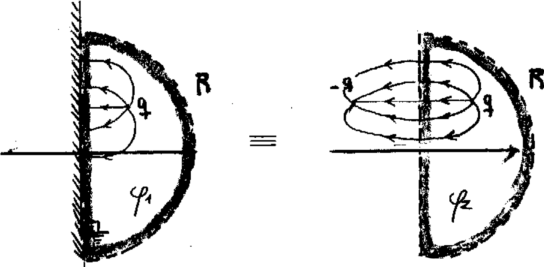
\includegraphics[width=0.6\textwidth]{images/fig_ft1_imagegreen1.pdf}	 
	\end{center}
	\caption{}
\end{figure} 

Los problemas que ilustra la figura satisfacen iguales condiciones de contorno en el recinto punteado,
entonces sus soluciones internas son la misma: $\phi_1 = \phi_2$ por unicidad.

\subsection{El Método de Green}

El concepto tras el método de Green es evaluar el $\phi$ de una carga puntual ante cierta configuración
de contornos conductores. Es una excitación elemental.

Restando entre sí
\[
	\Nabla\cdot(\phi\Nabla\psi) = \phi\lapm{\psi} + \Nabla\phi\cdot\Nabla\psi
\]
y
\[
	\Nabla\cdot(\psi\Nabla\phi) = \psi\lapm{\phi} + \Nabla\psi\cdot\Nabla\phi
\]
e integrando ambos miembros y utilizando el teorema de la divergencia, se llega a
\[
	\int_V \left[ \phi\lapm{\psi} - \psi\lapm{\phi}\right] dV =
	\int_S \left[ \phi\Nabla\psi - \psi\Nabla\phi \right] dS,
\]
que es la segunda identidad de Green.

Consideremos lo que llamaremos caso A, según vemos en figura, caracterizado según
\[
	\rho_{int} \qquad \vb{x}'\in R, \vb{x}\in R
\]
\begin{figure}[htb]
	\begin{center}
	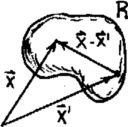
\includegraphics[width=0.3\textwidth]{images/fig_ft1_imagegreen2.pdf}	 
	\end{center}
	\caption{}
\end{figure} 
\[
	\psi = \frac{1}{|\vb{x}-\vb{x}'|} \qquad \lapm{\psi} = -4\pi \delta(\vb{x}-\vb{x}')
\]
\[
	-\phi(\vb{x})4\pi + \int_V 4\pi \frac{\rho(\vb{x}')}{|\vb{x}-\vb{x}'|} \; dV' =
	\int_S \left( \phi\dpar{\psi}{n}-\frac{1}{|\vb{x}-\vb{x}'|}\dpar{\phi}{n}\right)\; dS 
\]
donde estamos usando la abreviatura $\Nabla\phi\cdot\vb{n}=\partial\phi/\partial n$ que es la
derivada normal en la superficie.
\[
	,
\]


El caso B, según figura, corresponde a
\[
	\rho_{int} \qquad \vb{x}'\notin R, \vb{x}\in R
\]


\begin{figure}[htb]
	\begin{center}
	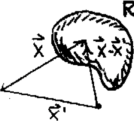
\includegraphics[width=0.3\textwidth]{images/fig_ft1_imagegreen3.pdf}	 
	\end{center}
	\caption{}
\end{figure} 

% =================================================================================================
\section{Funciones de Green}
% =================================================================================================

\begin{figure}[htb]
	\begin{center}
	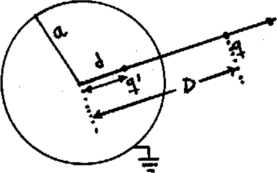
\includegraphics[width=0.6\textwidth]{images/fig_ft1_green1.pdf}	 
	\end{center}
	\caption{}
\end{figure} 

\begin{figure}[htb]
	\begin{center}
	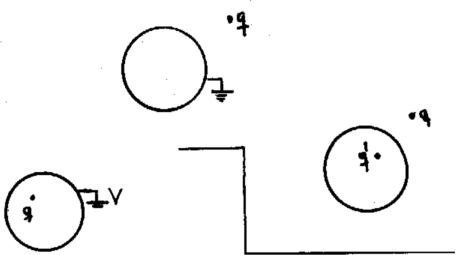
\includegraphics[width=0.6\textwidth]{images/fig_ft1_green2.pdf}	 
	\end{center}
	\caption{}
\end{figure} 



\begin{figure}[htb]
	\begin{center}
	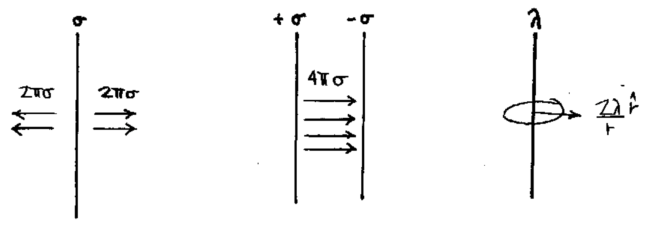
\includegraphics[width=0.6\textwidth]{images/fig_ft1_campohilos.pdf}	 
	\end{center}
	\caption{}
\end{figure} 


% \bibliographystyle{CBFT-apa-good}	% (uses file "apa-good.bst")
% \bibliography{CBFT.Referencias} % La base de datos bibliográfica

\end{document}
